\section{Results and Discussion} \label{sec:0result}
In this section, we evaluate the performance of the proposed control strategy through different simulation scenarios.

\subsection{Simulation setup}
In the simulation, the UAV has the alert radius $r_a = 0.3$ m and the sensing radius $r_s = 2$ m. The control period is set at $0.02$ s. The maximum speed of each UAV is $2.0 \text{ m/s}$. The V-shape formation is defined with $d=0.8 \text{ m}$ and $\alpha=0.3\pi/4 \text{ rad}$. In our evaluation, 5 UAVs with V-shape formation are operated in the area of 46 m $\times$ 7 m with two large obstacles arranged to form a narrow passage as shown in Figure \ref{fig:chap2_result}.

\subsection{Results}
\begin{figure*}
    \centering
    \begin{subfigure}[b]{\textwidth}
        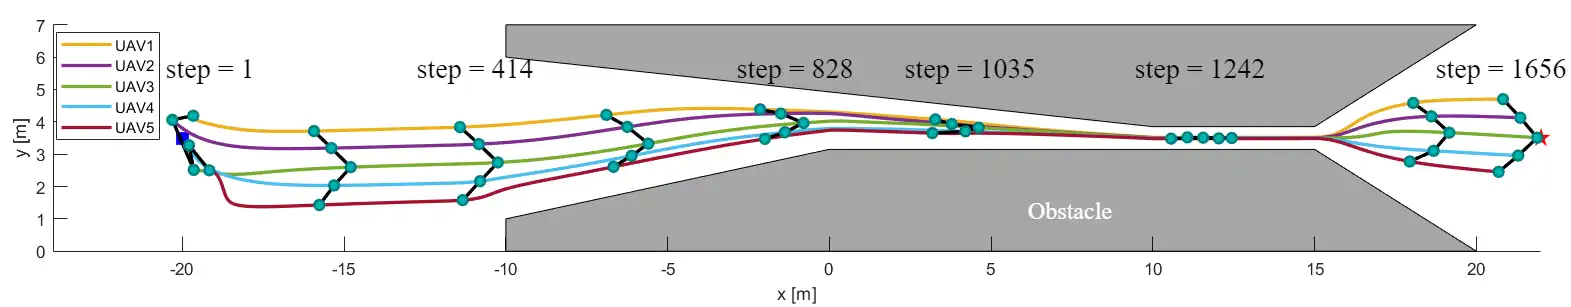
\includegraphics[width=\textwidth]{paper1/images/result.png}
        \caption{Trajectories of the UAVs in the formation}
        \label{fig:chap2_motion}
    \end{subfigure}
    \begin{subfigure}[b]{\textwidth}
        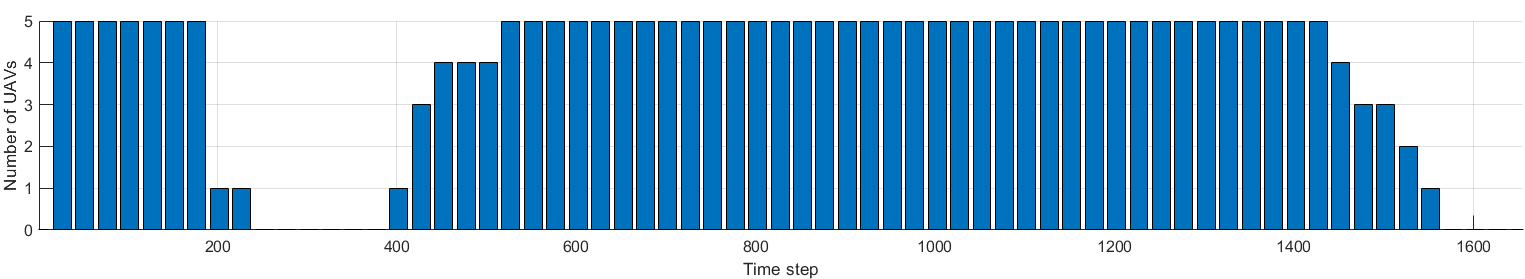
\includegraphics[width=\textwidth]{paper1/images/number.png}
        \caption{Number of UAVs activating reconfiguration behaviors over time}
        \label{fig:chap2_number}
    \end{subfigure}
    \caption{Simulation result of the V-shape formation moving through a narrow passage}
    \label{fig:chap2_result}
\end{figure*}

\begin{figure*}[t]
    \centering
    \begin{subfigure}[b]{0.495\textwidth}
    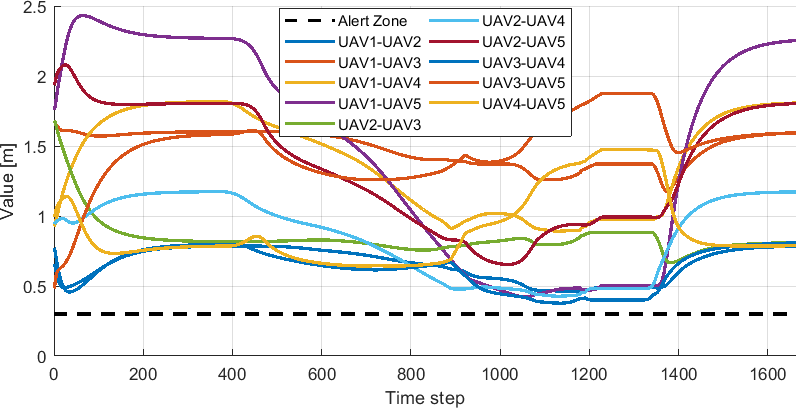
\includegraphics[width=\textwidth]{paper1/images/distance.png}
    \caption{Distances between each pair of UAVs over time}
    \label{fig:chap2_distance}
    \end{subfigure}
    \begin{subfigure}[b]{0.495\textwidth}
    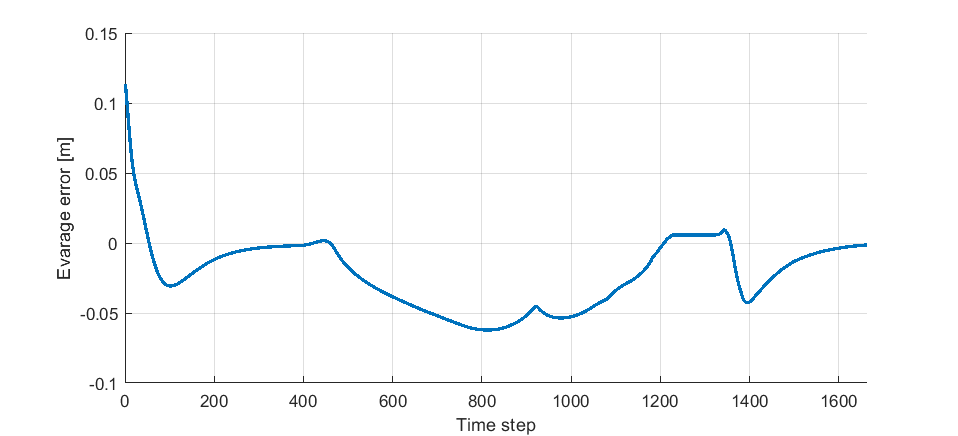
\includegraphics[width=\textwidth]{paper1/images/error.png}
    \caption{The average distance error of UAV formation}
    \label{fig:chap2_error}
    \end{subfigure}
    \begin{subfigure}[b]{0.495\textwidth}
    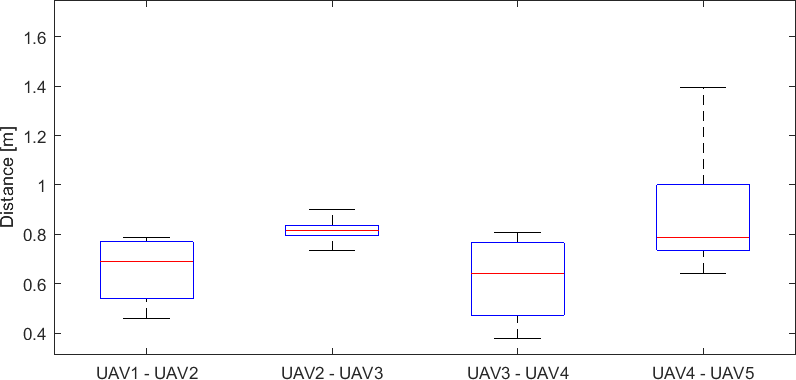
\includegraphics[width=\textwidth]{paper1/images/mean.png}
    \caption{The distance between consecutive UAVs}
    \label{fig:chap2_mean}
    \end{subfigure}
    \begin{subfigure}[b]{0.495\textwidth}
    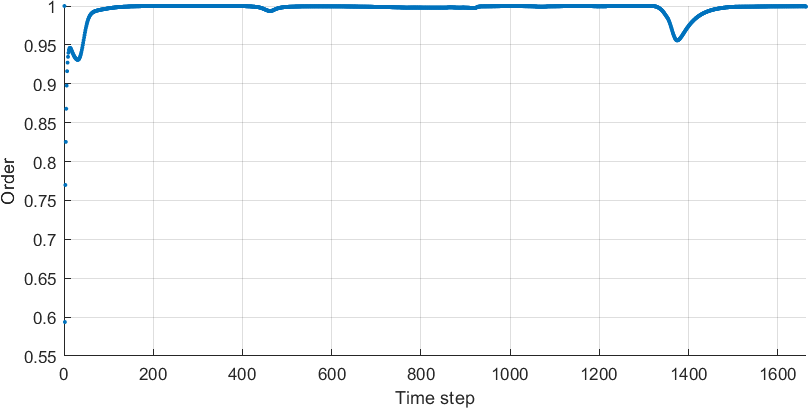
\includegraphics[width=\textwidth]{paper1/images/heading.png}
    \caption{Values of the \textit{order} metric $\Phi$ over time}
    \label{fig:chap2_heading}
    \end{subfigure}
    \caption{Evaluation of the proposed algorithm}
    \label{fig:chap2_eval}
\end{figure*}

\begin{table*}[!]
\centering
\caption{Statistical evaluation of the proposed strategy for several different scenarios}
\label{tbl:chap2_sta}
\begin{tabular}{C{0.8cm}C{1.5cm}C{1cm}C{1cm}C{2cm}C{2.5cm}C{4.0cm}}
\hline
Scen. & Number UAVs & $d$ & $\alpha$    & Average error (m) & Min distance (m) & Average distance of consecutive UAVs (m) \\ \hline
1     & 3        & 1.0   & $3\pi/4$             & 0.12333   & 0.48557   & 0.98788                      \\
2     & 5        & 1.0   & $3\pi/4$    & 0.12068   & 0.37383   & 0.96575                      \\
3     & 3        & 0.8   & $5\pi/6$    & 0.10942   & 0.48988   & 0.87599                      \\
4     & 3        & 1.0   & $4\pi/5$    & 0.13666   & 0.47581   & 1.0943                       \\
5     & 5        & 0.8   & $3\pi/4$    & 0.111     & 0.41279   & 0.88913     \\ \hline                
\end{tabular}
\end{table*}

Figure \ref{fig:chap2_result} shows the trajectories of the UAVs moving in the environment under the guidance of the proposed distributed controller. Initially, the UAVs are randomly positioned around a starting point (step 1). They then self-adjust to form the desired V-shape formation (step 414) based on the control signals generated by the formation and reconfiguration behaviors. As they encounter obstacles, the UAVs start to adjust their formation. This includes deforming the formation (steps 414-1035) and transitioning to a straight-line formation (step 1242) to navigate through narrow gaps. Upon successfully circumventing the obstacles, the UAVs readjust to form the desired V-shape and proceed toward the goal position (step 1656). The result can be verified in the simulation video shown in the footnote\footnote{Simulation video: {\fontfamily{qcr}\selectfont
\url{https://youtu.be/_6u7yMNOySc}}}. 

Figure \ref{fig:chap2_number} shows the number of UAVs activating their reconfiguration behavior over time. It can be seen that the UAVs activate this behavior when shaping the formation at the initialization stage, and during the process of adjusting their formation to adapt to the environment structure.

The statistical results of the evaluation of the proposed strategy are depicted in Figure \ref{fig:chap2_eval}. Figure \ref{fig:chap2_distance} shows the distances between the UAVs over time. It can be seen that those distances are all greater than the alert radius, which confirms the effectiveness of the control algorithm in avoiding collision among the UAVs.

Figure \ref{fig:chap2_error} presents the average distance error of the UAV formation over time. Initially, the error is large since the UAVs have not formed the desired shape. After the control algorithm realigns the UAV to their desired positions, the error quickly converges toward zero. While the formation navigates through the narrow passage, the error remains small, less than $0.06$ m. Figure \ref{fig:chap2_mean} shows the average distance between consecutive UAVs. It can be seen that the average distance fluctuates around the desired value for the V-shaped formation ($d=0.8$ m), which is desirable for the formation.

To further evaluate the performance of the proposed controller, an \textit{order} metric $\Phi$ that measures the similarity in the UAVs' direction is used \cite{Vicsek1995}. It takes the values in range $[0, 1]$ and is computed as follows:
\begin{equation}
    \Phi=\dfrac{1}{n}\left\Vert\sum_{i=1}^n{\left[\cos\psi_i, \sin\psi_i\right]^T}\right\Vert.
    \label{eq:order}
\end{equation}

According to (\ref{eq:order}), the order metric $\Phi$ is close to 1 when all UAVs have the same heading angle. Figure \ref{fig:chap2_heading} shows the value of $\Phi$ in our simulation. It can be seen that $\Phi$ is close to 1 during the movement of the formation, even when the formation avoids obstacles or traverses through a narrow passage. Changes in the heading angle increase when exiting the passage since the UAVs in the formation need to realign to the origin shape. However, the order metric then quickly converges to 1 when the UAVs form their desired formation. The results thus confirm the validity of the proposed control algorithm.

%\subsection{Discussion}
To further evaluate the performance of the proposed method, simulations on various scenarios such as narrow passages of varying widths and dense obstacle areas have been conducted. In addition, the number of UAVs and V-shape parameters, the desired distance, $d$, and the desired bearing angle, $\alpha$, are also varied. The results, including the average formation error, the closest distance between two UAVs, and the average distance between consecutive UAVs, are summarized in Table {\ref{tbl:chap2_sta}}. It is evident that the average formation error approximates $0.1$~m, which is sufficient for the formation to maneuver in narrow spaces. Furthermore, the minimum distance between any pair of UAVs is larger than the collision threshold, $r_a$, and thus meets the requirement for collision avoidance. Finally, the average distance between consecutive UAVs closely aligns with the desired value, indicating the stability in the formation shape. These results confirm the validity and effectiveness of our proposed control strategy.